\pgfplotsset{compat=1.18} 
\usetikzlibrary{calc}
\usepgfplotslibrary{groupplots}
\begin{figure*}[t!]
\vspace{-2em}
\centering
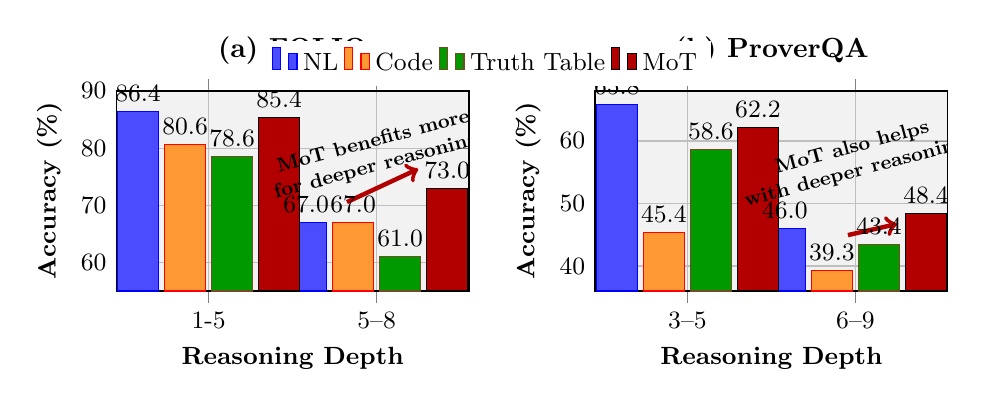
\begin{tikzpicture}
\begin{groupplot}[
    group style={
        group size=2 by 1,
        horizontal sep=1.6cm
    },
    ybar,
    % bar width=18pt,
    % width=0.5\textwidth,
    height=5cm,
    axis background/.style={fill=gray!10},
    enlarge x limits=0.46,
    grid=major,
    tick label style={font=\small},
    label style={font=\small},
    nodes near coords,
    % every node near coord/.append style={font=\small, black},
    every node near coord/.append style={
            font=\small,
            black
        },
        point meta=explicit symbolic,
    legend style={
        at={(0.33,1.25)},
        % anchor=south west,
        legend columns=4,
        draw=none,
        font=\small
    }
]

% ----------- 第一个图：FOLIO -----------
\nextgroupplot[
    title={\textbf{(a) FOLIO}},
    width=0.5\textwidth,
    height=0.34\textwidth,
    ymin=55, ymax=90,
    enlarge x limits=0.55,
    bar width=15pt,
    xlabel={\textbf{Reasoning Depth}},
    ylabel={\textbf{Accuracy (\%)}},
    symbolic x coords={1-5, 5--8},
    xtick=data
]
    \addplot+[fill=blue!70] coordinates {(1-5,86.4) [86.4] (5--8,67.0) [67.0]};
    \addplot+[fill=orange!80] coordinates {(1-5,80.6) [80.6] (5--8,67.0) [67.0]};
    \addplot+[fill=green!60!black] coordinates {(1-5,78.6) [78.6] (5--8,61.0) [61.0]};
    \addplot+[fill=red!70!black] coordinates {(1-5,85.4) [85.4] (5--8,73.0) [73.0]};

    \node[align=center, font=\small, text=black, rotate=15, scale=0.8] at (axis cs:5--8,79)
        {\textbf{MoT benefits more}\\\textbf{for deeper reasoning.}};

    \coordinate (motStartF) at (axis cs:1-5,75.4);
    \coordinate (motEndF) at (axis cs:5--8,72.0);
    \draw[->, ultra thick, red!70!black]
        ($(motStartF)+(50pt,-10pt)$) -- ($(motEndF)+(15pt,9pt)$);

% ----------- 第二个图：ProverQA -----------
\nextgroupplot[
    title={\textbf{(b) ProverQA}},
    width=0.5\textwidth,
    height=0.34\textwidth,
    ymin=36, ymax=68,
    enlarge x limits=0.55,
    bar width=15pt,
    xlabel={\textbf{Reasoning Depth}},
    ylabel={\textbf{Accuracy (\%)}},
    symbolic x coords={3--5, 6--9},
    xtick=data
]
    % \addplot+[fill=blue!70] coordinates {(1-2,86.2) [84.3] (3--5,65.8) [68.5] (6--9,46.0)};
    % \addplot+[fill=orange!80] coordinates {(1-2,51.4) [79.2] (3--5,45.4) [65.8] (6--9,39.3) [65.8]};
    % \addplot+[fill=green!60!black] coordinates {(1-2,82.4) [77.5] (3--5,58.6) [60.1] (6--9,43.4)};
    % \addplot+[fill=red!70!black] coordinates {(1-2,83.2) [83.7] (3--5,62.2) [74.9] (6--9,48.40)};

    \addplot+[fill=blue!70] coordinates { (3--5,65.8) [65.8] (6--9,46.0)[46.0]};
    \addplot+[fill=orange!80] coordinates { (3--5,45.4) [45.4] (6--9,39.3) [39.3]};
    \addplot+[fill=green!60!black] coordinates {(3--5,58.6) [58.6] (6--9,43.4)[43.4]};
    \addplot+[fill=red!70!black] coordinates { (3--5,62.2) [62.2] (6--9,48.40) [48.4]};

    \node[align=center, font=\small, text=black, rotate=15, scale=0.8] at (axis cs:6--9,57)
        {\textbf{MoT also helps}\\\textbf{with deeper reasoning.}};

    \coordinate (motStartPQ) at (axis cs:3--5,50.7);
    \coordinate (motEndPQ) at (axis cs:6--9,60);
    \draw[->, ultra thick, red!70!black]
        ($(motStartPQ)+(58pt,-13pt)$) -- ($(motEndPQ)+(15pt,-30pt)$);

\legend{NL, Code, Truth Table, MoT}
\end{groupplot}
\end{tikzpicture}
\vspace{-1em}
\caption{\footnotesize{Performance comparison of different thought paradigms across reasoning depths. On FOLIO and ProverQA benchmarks, MoT inference exhibits better performance on difficult problems.}}
\vspace{-1em}
\label{fig:group-mot-depth}
\end{figure*}
